\chapter{Background} \label{chapter:background}

\begin{figure}[!tbp]
	\centering
	\begin{minipage}[t]{0.45\textwidth}
		\centering
    	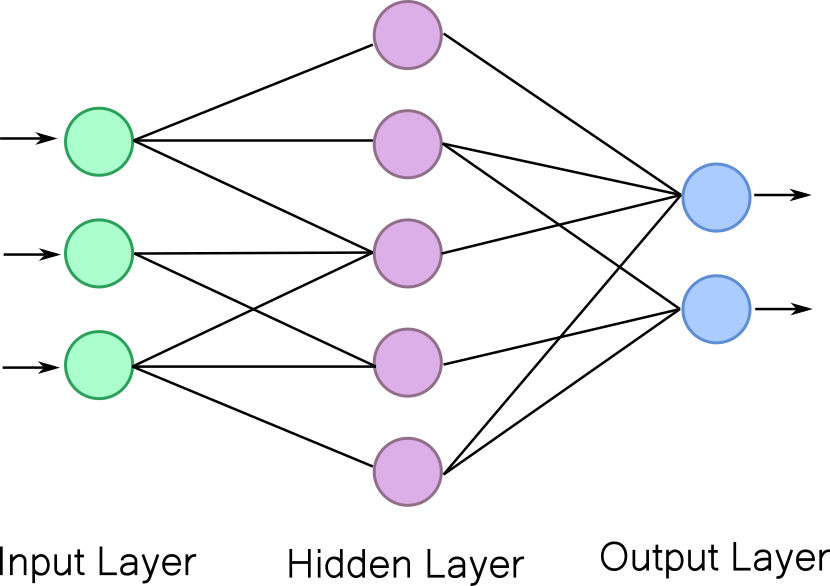
\includegraphics[width=0.8\linewidth]{ffnn}
    	\caption{Abstract structure of a feed-forward neural network. Most networks have more layers and more neurons per layer.}
    	\label{fig:ffnn}
    \end{minipage}
	\hfill
	\begin{minipage}[t]{0.45\textwidth}
		\centering
		\begin{tikzpicture}[scale=0.5, transform shape]
  			\begin{axis}[scale only axis,
    					axis lines=middle,
    					inner axis line style={=>},
    					xlabel={},
    					ylabel={},
    					ytick={-1,-0.5,...,1},
    					xtick={-1,-0.5,...,1},
    					ymin=-1,
    					ymax=1,
    					xmin=-1,
    					xmax=1
  						] 
    			\addplot [mark=none,  blue,   ultra thick] {max(0, x)}; 
  			\end{axis}
		\end{tikzpicture}
    	\caption{Visualization of the \ac{relu} activation function $f(x) = \max(0, x)$.}
    	\label{fig:relu}
    \end{minipage}
\end{figure} 

\section{Neural Networks}

The following sections dissect the individual components of a neural network and explain concepts and procedures. 

\subsection{Neuron}

A \textit{Neuron} is the smallest atomic unit of a neural network. The layers of a network consist of neurons. A neuron computes the linear function 

\begin{align}
y = \sum\limits_{i=0}^kw_ix_i + b
\end{align}

\noindent where $w_i$ is the weight for the $i$-th input $x_i$ and $b$ is a bias. The weights and the bias are the values that can be learned during the training process of the network (see Section \ref{section:network_training}). The output of a layer of the network is the vector $(y_0, \cdots, y_t)$, $y_j$ being the output of the $j$-th neuron. Those outputs then serve as inputs to the next layer, i.e. $y_i$ becomes $x_i$. Not every output has to be used by every next neuron. To prevent the network from collapsing into a single linear classifier and thus to increase the expressivity of the network, the output of a neuron is put into a non-linear so-called activation function. Although many different activation functions exist, most popular is the \textit{\ac{relu}}, which was first presented by Jarrett et al. in \cite{relu}. The function is exemplarily visualized in \fig \ref{fig:relu} and is calculated as

\begin{align}
f(x) = \max(0, x)
\end{align} 

\subsection{Feed-Forward Neural Networks}

A \textit{Feed-Forward Neural Network} is a network consisting of layers of neurons. The first layer is called the input layer. Those are the neurons that receive the data that the network is supposed to process. The last layer is called the output layer. The form of the output of the neural network depends on the field of application. It can be object coordinates like in our case, class probabilities in classification tasks or any other real-valued output. The intermediate layers are called hidden layers. Their number can grow to over a hundred in modern networks \cite{resnet}, thus the name deep neural networks. All layers can have different numbers of neurons and connections to previous layers. A layer, in which each neuron is connected  to every output of the previous layer using individual weights for each connection, is called a \textit{Fully-Connected Layer}. A schematic overview over the structure of a neural network is visualized in \fig \ref{fig:ffnn}. The green circles on the left are the neurons of the input layer. The purple neurons in the middle belong to intermediate (hidden) layers. The output layer consists of the blue neurons on the right. A neural network can generally be seen as the function $y=f(x,\theta)$, where $\theta$ are the weights and biases of the neurons and $y$ is the output of the network.

\subsection{Convolutional Neural Networks}

\begin{figure}[!tbp]
	\centering
	\begin{subfigure}[t]{0.45\textwidth}
		\centering
    	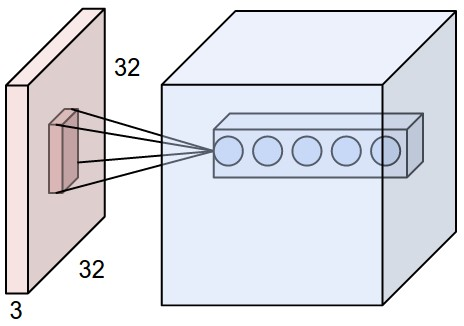
\includegraphics[width=0.7\linewidth]{conv_layer}
    	\caption{Example convolutional layer. The input image has dimensions 32x32 and 3 channels. The blue volume is the actual convolutional layer with multiple filters. Image from \cite{convolutional_layer_image}.}
    	\label{fig:conv_layer}
	\end{subfigure}
	\hfill
	\begin{subfigure}[t]{0.5\textwidth}
		\centering
    	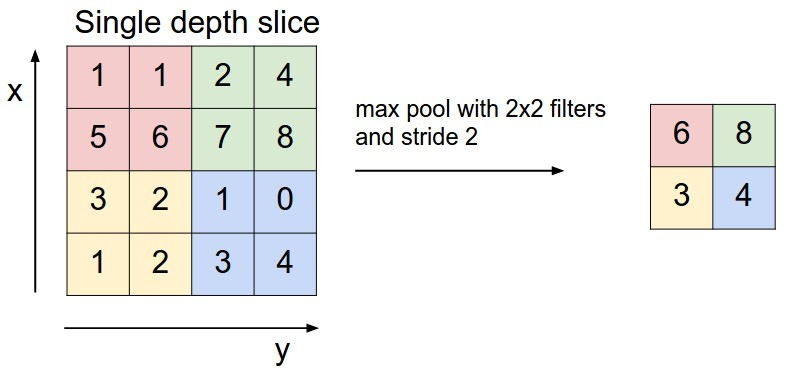
\includegraphics[width=0.9\linewidth]{pool_layer}
    	\caption{Example pooling layer with maximum as pooling operation. Image from \cite{pooling_layer_image}.}
    	\label{fig:pool_layer}
	\end{subfigure}
	\caption{The two main layer types of a convolutional neural network.}
\end{figure} 

Depending on its depth and number of neurons, a densely connected feed-forward network with individual weights for each neuron needs a lot of memory and computation time to perform operations. A \textit{\acf{cnn}} reduces this need for memory and increases computational throughput by sharing the weights of the neurons. This type of network is often employed in computer vision tasks, like image classification and segmentation. A \ac{cnn} introduces two new types of layers: \textit{Convolutional Layers} and \textit{Pooling Layers}. A convolution layer convolves the input using a kernel. This means that the kernel is moved along the input's dimensions and sums up the respective values multiplied by the kernel weights. For a position $(i, j)$ in the input $I$ and a kernel matrix $K$, this can be written as

\begin{align}
O(i, j) = \sum\limits_{w_0, w_1} I(i + w_0, j + w_1)K(i + w_0, j + w_1) \label{eqn:convolutional_layer}
\end{align} 

where $O$ is the output. The ranges of $w_0$ and $w_1$ depend on the size of the convolution window.
The kernel can be learned but stays the same for the whole convolution. \fig \ref{fig:conv_layer} shows an abstraction of a convolutional layer. The red plane on the left is the input image, the blue cube on the right is the actual layer. The blue cube is broader than the red input because it has multiple filters. Each filter consists of an independent kernel. This means that this layer has multiple outputs, each being a convolution of the input with a different kernel.

A pooling layer can be used to reduce the size of the data between convolution layers. This significantly speeds up computation and reduces memory consumption. It also reduces the number of parameters which helps to prevent the network from overfitting. An overfitted network performs well on the data it was trained on but does not generalize well, i.e. has a significantly lower accuracy on unseen data. A pooling layer alters equation \ref{eqn:convolutional_layer} in the following way:

\begin{align}
O(i, j) = \max\limits_{w_0, w_1} I(i + w_0, j + w_1)
\end{align} 

The size of the output of the pooling layer is reduced by a factor depending on the size of the pooling window.

\subsection{Network Training} \label{section:network_training}

A network's weights and biases can be initialized to 0 or sampled randomly from a Gaussian distribution. To set the parameters to meaningful values that produce the desired output, we need to train the network. The following paragraphs describe techniques to train a network.

\subsubsection{Error-Back Propagation} The predominant procedure to train a network is called \textit{Error-Back-Propagation} or \textit{Backpropagation}. To employ backpropagation, a differentiable but arbitrary loss function has to be defined. The loss function measures the error of the output of the network compared to the desired output, e.g. by summing up the squared differences of the output and the objective output. The term \textit{loss} and \textit{error} or \textit{error rate} stand for the same thing. First, the network is applied to a training example in the so-called forward pass. Next, the loss function is derived with respect to each weight of the network. The derivative, the computed and the desired output together yield the delta to be applied to the weights. This delta is then also propagated backwards through the net and the deltas of the layers in between are calculated using the chain rule of calculus. After the deltas for all neurons have been computed, the weights are updated according to an update rule. We explain some of these rules in the next paragraph. 

\subsubsection{Optimization} There exist many different patterns how to update the network weights after obtaining the deltas. The \textit{\ac{sgd}} multiplies the delta by a learning rate and subtracts it from the weight. To ensure convergence, the learning rate is often decreased over time. A more elaborate method is the \textit{Adaptive Moment Optimization (Adam)} \cite{adam} which computes adaptive learning rates for each parameter. The algorithm computes and stores an exponentially decaying average over past gradients as well as an exponentially decaying average over the past squared gradients. This serves to increase the learning rate in case of small gradients and decrease the learning rate in case of large gradients. Both averages are stored for the next iteration. There exist other optimization procedures that are not covered here.
	
\subsubsection{Regularization} Regularization can mean various things for neural networks. In general, its purpose is to keep the network from overfitting. Ian Goodfellow defined it in \cite{goodfellow} as any modification that reduces the generalization error but not the training error. Many network architectures regularize the network by adding a penalty term on the weights. Another possibility is to randomly deactivate a subset of the neurons to force the network to adapt to this loss of information. This is called \textit{Dropout}. \textit{Batch Normalization} helps the network generalize by subtracting the batch mean and batch standard deviation from the output of the previous layer. A batch is a subset of the input data. This technique typically speeds up network training and allows running the network on a machine that can't fit the whole dataset in its memory. To keep \ac{sgd} or other optimizers from reversing the covariance shift performed by batch normalization, the two parameters \textit{beta} and \textit{gamma} of such a layer are usually trainable. This way, a layer of neurons cannot fully counterpoise the shift. 

\section{6D Pose Estimation}

\begin{figure}[!tbp]
	\centering
	\begin{subfigure}[t]{0.29\textwidth}
		\centering
    	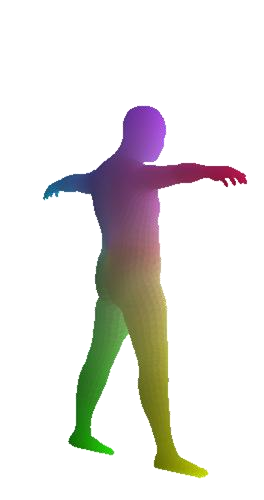
\includegraphics[width=0.45\linewidth]{human_object_coordinates}
    	\caption{The object coordinate representation of a human. Image from \cite{tsharp}.}
    	\label{fig:human_object_coordinates}
	\end{subfigure}
	\hspace{5mm}
	\begin{subfigure}[t]{0.29\textwidth}
		\centering
    	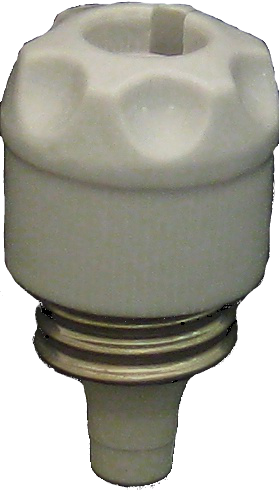
\includegraphics[width=0.45\linewidth]{tless_object}
    	\caption{An example object from the T-Less dataset. Image from \cite{tless}.}
    	\label{fig:tless_object}
	\end{subfigure}
	\hspace{5mm}
	\begin{subfigure}[t]{0.29\textwidth}
		\centering
    	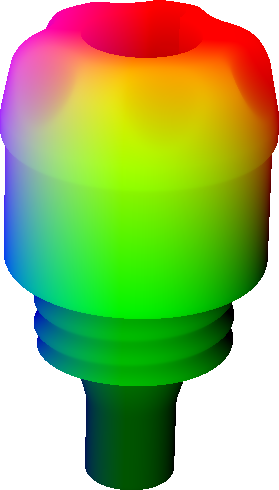
\includegraphics[width=0.45\linewidth]{tless_object_coordinates}
    	\caption{The corresponding rendered 3D object coordinates (scaled for visualization).}
    	\label{fig:tless_object_coordinates}
	\end{subfigure}
	\caption{Example 3D coordinate representations.}
\end{figure} 

\textit{6D pose estimation} is a central task in the computer vision community. The goal is to retrieve the translation and rotation of an object relative to the camera. 6D refers to the \textit{\ac{6dof}}, i.e. the 6 free parameters of the 3D translation and 3D rotation. The field of application ranges from medical imaging, robotics, augmented reality and many more.

There are different possible ways to estimate the pose with learning-based approaches. The 6 parameters can be predicted directly or an intermediate representation can be used for pose computation. Predicting the parameters offers no possibility to verify or improve the pose afterwards. A possible intermediate representation are object coordinates. This means that the 3D locations on the object are predicted for the 2D pixels in the input image. Each subset of object coordinates leads to a certain pose. The next section will introduce this concept of object coordinates in depth.

\subsection{Object Coordinate Regression} \label{objectcoordinates}

Tayler \etal first used object coordinates in \cite{tsharp}. Instead of directly predicting the location of joints or limbs of the human body, they computed the corresponding 3D location on the person for each pixel (see \fig \ref{fig:human_object_coordinates}). This idea can be transfered to objects of any kind. \fig \ref{fig:tless_object} shows an example object from the T-Less dataset \cite{tless} and \fig \ref{fig:tless_object_coordinates} shows the corresponding rendered 3D object coordinates.

The 2D-3D correspondences between object coordinates and pixels yield the \textit{\ac{pnp} Problem}. For a given 2D location $u$ in the image and the corresponding 3D point $p$, a pose consisting of the rotation matrix $R$ and the translation vector $t$ has to fulfill the equation

\begin{align}
 u = K \ [ \ R \ | \ t \ ] \ p \label{eq:pose_projection}
\end{align} 
 
\noindent where $K$ is the camera matrix

\begin{align}
K = \begin{bmatrix}
f_x & s & c_x \\
0 & f_y & c_y \\
0 & 0 & 1 
\end{bmatrix}
\end{align}

\noindent which projects the 3D point transformed into the camera coordinate system on the 2D image plane. The points $u$ and $p$ are both in homogeneous coordinates, i.e. $u = \begin{bmatrix} u \\ v \\ 1 \end{bmatrix}$ and $p = \begin{bmatrix} X \\ Y \\ Z \\ 1 \end{bmatrix}$. The skew factor $s$ is usually $0$. The principal point $(c_x, c_y)$ normally is the center of the image and $f_x$ and $f_y$ are the focal lengths in $x$ and $y$ direction, respectively. The values for those variables can vary, for example when cropping the image. \fig \ref{fig:pnp} visualizes the relation of pixels and object coordinates. If equation \ref{eq:pose_projection} is overdetermined because there are more correspondences than variables, it cannot be solved directly.

\begin{figure}[!tbp]
	\centering
    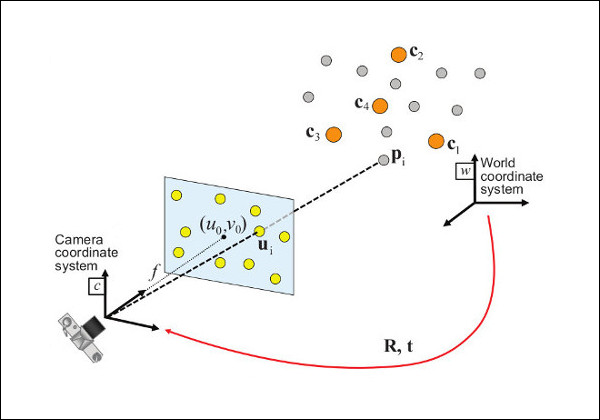
\includegraphics[width=0.45\linewidth]{pnp}
    \caption{The relationship between the camera, the 3D points and their projections on the screen defined by the rotation matrix $R$ and the translation vector $t$. Image from \cite{opencv_pnp}.}
    	\label{fig:pnp}
\end{figure} 

A method to solve the \ac{pnp} problem for many correspondences is to use the \textit{\ac{ransac} algorithm} \cite{ransac}. \ac{ransac} selects a model based on a subset of the dataset and evaluates it using an energy function. This way, the approximate best model is found iteratively. Algorithm \ref{algorithm:ransac} shows the outline of the \ac{ransac} algorithm for pose estimation. The energy function can be arbitrary but should capture the quality of the pose. For example, the number of inliers can be counted. An inlier is a 3D point whose reprojection error is within a certain threshold.

\begin{algorithm}
\caption{\ac{ransac}} \label{algorithm:ransac}
\begin{algorithmic} 
\REQUIRE Set of 3D points
\REQUIRE Set of corresponding 2D points
\REQUIRE Number of iterations $i$
\REQUIRE An energy function to score the pose hypothesis $E$
\STATE Set current energy $e=0$
\STATE Set current best pose hypothesis $H*$ = $null$
\FOR{$1 ... i$}
\STATE Select a subset of corresponding 2D and 3D points to compute pose $H$
\STATE Compute energy $e'$ of pose $H$: $e'=E(H)$
\IF{$e' > e$}
\STATE $H* = H$
\STATE $e = e'$
\ENDIF
\ENDFOR
\RETURN Best pose $H*$
\end{algorithmic}
\end{algorithm}